\documentclass{article}
\usepackage[english]{babel}
\usepackage[a4paper,top=2cm,bottom=2cm,left=3cm,right=3cm,marginparwidth=1.75cm]{geometry}
\usepackage{listings}
\lstset{
  basicstyle=\ttfamily,
  columns=fullflexible,
  frame=single,
  breaklines=true,
  postbreak=\mbox{\textcolor{red}{$\hookrightarrow$}\space},
}
% Useful packages
\usepackage{amsmath}
\usepackage{graphicx}
\usepackage[colorlinks=true, allcolors=blue]{hyperref}
\usepackage{makecell}
\usepackage[utf8]{inputenc}
\usepackage{csquotes}

\usepackage[T1]{fontenc}

\usepackage{lmodern}
\usepackage[
backend=biber,
style=numeric-comp,
]{biblatex}
\addbibresource{references.bib}


\title{Conversational Drive Through Restaurant Dataset\: Prompt Engineering with GPT \& Gemini}
\author{Aaron Fletcher \& Boxuan Shaun}

\begin{document}
\maketitle
\section{Introduction}
Prompt engineering is the process of modifying the input of a model to achieve optimal results. In the case of large language models (LLMs), the prompt is a textual sequence indicating a task the model should perform, such as "In computer science, what is priority inversion?" - see Figure \ref{fig:priority-engineering}. Given this initial prompt, the information recovered from the LLMs will generally complete the task. However, it may not be in line with the intended audience. Engineering this prompt with modifiers can ensure that the response matches this target audience, such as "Respond in a way that a 5-year-old would understand: In computer science, explain what priority inversion is?" - see Figure \ref{fig:5-yo-prompt}.

An emerging property of LLMs enables prompt engineering: in-context learning (ICL). ICL is the ability of a language model to make inferences based on information provided with the input, typically preceding or following it. In the above example, given the proceeding prompt "Respond in a way that a 5-year-old would understand," the LLM would not update its parameters and respond using its pre-trained model but the context to shape the response.

\begin{figure}
    \centering
    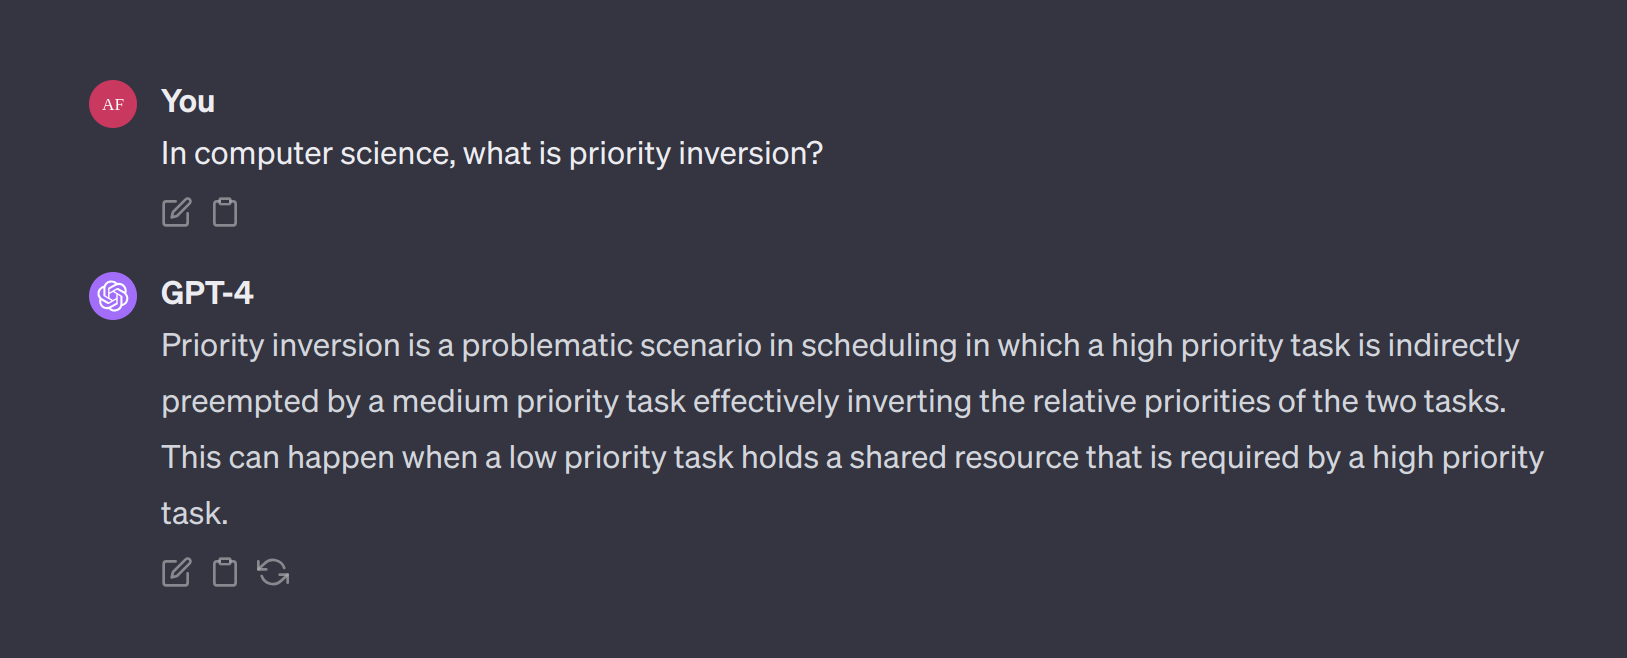
\includegraphics[width=1\linewidth]{sections//images/what-is-priority-inversion.png}
    \caption{Chat GPT asked a standard computer science question, using GPT 4.5}
    \label{fig:priority-engineering}
\end{figure}

\begin{figure}
    \centering
    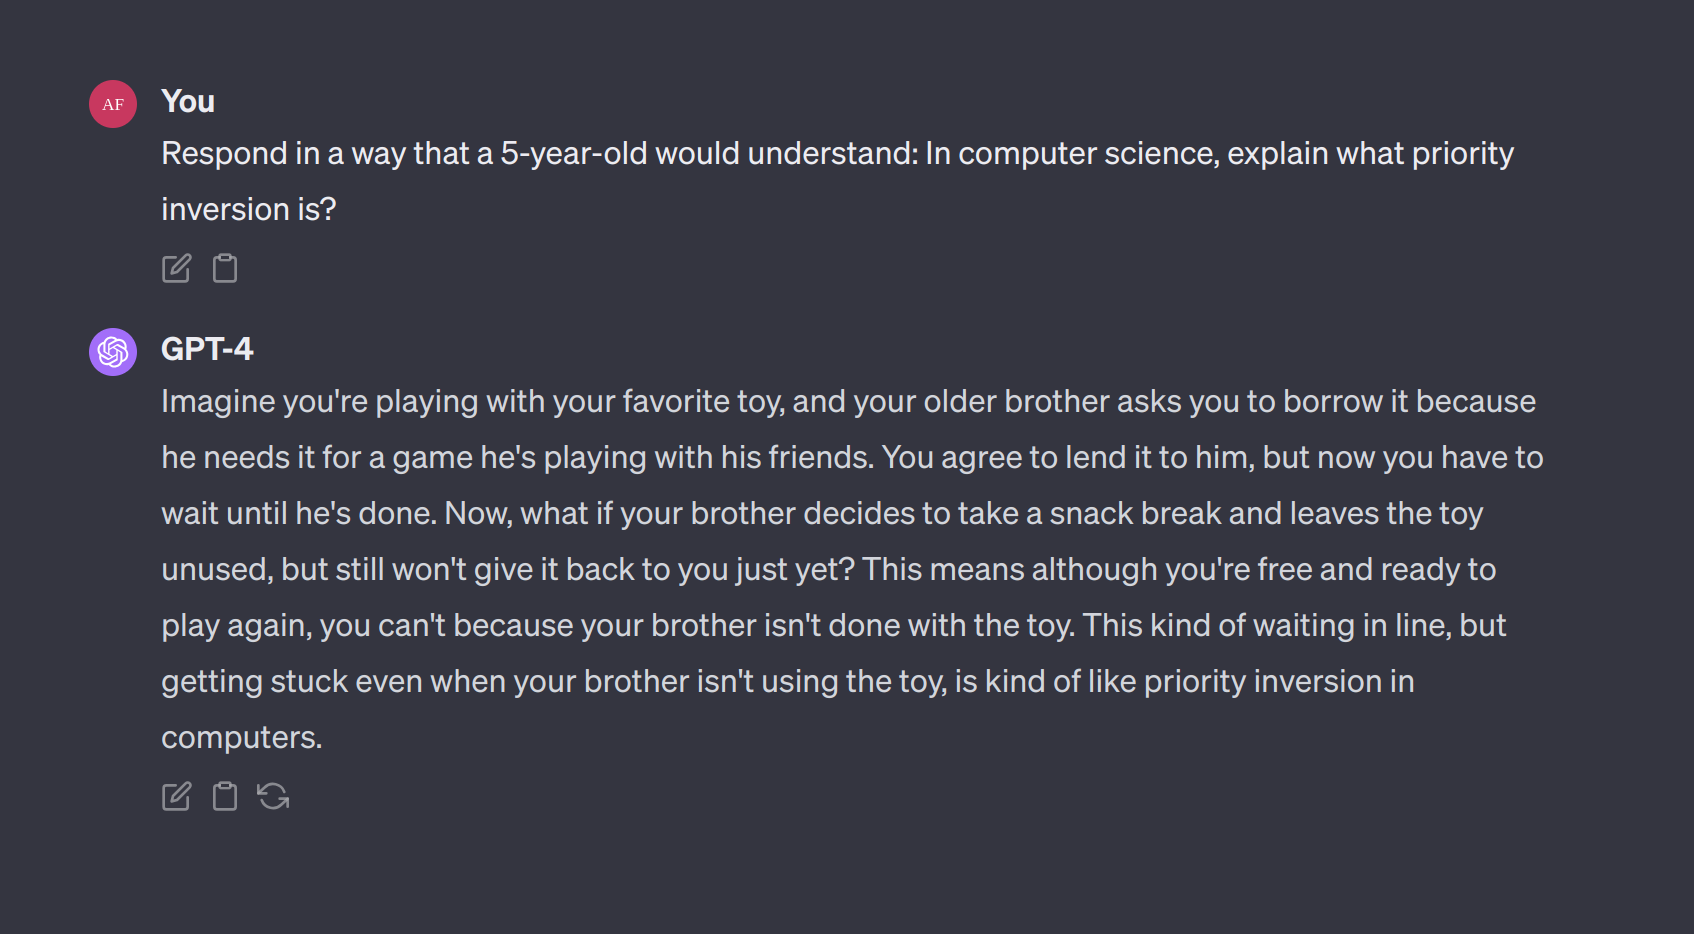
\includegraphics[width=1\linewidth]{sections//images/5-year-old-priority-inversion.png}
    \caption{Chat GPT asked a standard computer science question, with prompt engineering, using GPT 4.5}
    \label{fig:5-yo-prompt}
\end{figure}

Recently, Google released a new generative model, reportedly superior to the GPT-4 architecture, the Gemini model, in November 2023. Little research exists to evaluate the effect of prompt engineering on Gemini architecture.  

This research aims to understand whether prompt engineering improves the effects of downstream tasks presented within this mini-project and additionally establish some prompt-engineering performance comparison of GPT-4 to the Gemini model. 
\newpage
\section{Related Works}
There exists multiple research studies investigating the effects of prompt engineering on LLMs \cite{van_zandvoort_enhancing_2023, lee_cxr-llava_2023, chen_unleashing_2023}. 

\textbf{Definitions: }
\begin{itemize}
    \item One-Shot Learning - The ability of a LLM to learn from a limited dataset, with one example per class \cite{o_mahony_one-shot_2019}.
    \item Few-Shot Learning - The same as one-shot learning but with multiple examples per class \cite{parnami_learning_2022}.
    \item Chain-of-thought reasoning (COTR) is a that parallels human reasoning \cite{wei_chain--thought_2022}. This technique prompts the model to break down the problem into multiple steps before giving a final answer. COTR is a type of few-shot learning.
    \item ROLE PLAY PROMPTING

\end{itemize}




\newpage
\section{Experimental Approach}
At its core, this project aims to use audio data to represent ordered items accurately. The experimental design generates three forms of data: the scenario audio, a human-validated transcribed representation of the scenario, and the finalised ordered items.

Prompt engineering can occur any time data are being passed to a model. Audio prompting is enabled by using OpenAI's whisper model's API, which allows textual information to be supplied to the model to improve its performance. Notably, only 224 tokens can be provided to the model, with any preceding tokens ignored. Textual prompt engineering can be achieved by modifying the textual input through prepending, extending, or modifying the input.  


Due to API limitations, the audio files were pre-processed into 25 MB or smaller files and fed into the transcription API. These transcriptions can be concatenated to form a larger transcription.

\subsubsection{Inclusion/Exclusion Critera}
All calls to the API will follow the same parameters, as shown in Table \ref{tab:standard_params}.

In cases where the textual prompts exceed the token limits of one of the tested models, that data will be removed from that experiment.



\begin{table}[ht]
    \centering
    \begin{tabular}{|c|c|c|c|}
        \hline - & \textbf{Whisper} & \textbf{Gemini}  & \textbf{GPT} \\
        \hline Version & whisper-1  &  Gemini Pro & gpt-4-1106-preview \\
        \hline Size/Token Limit & 25mb  & 32000 Tokens & 128000 Tokens \\
        \hline API Endpoint & - & - & - \\   
        \hline Input Format & mp3 & text & text \\
  \hline

    \end{tabular}
    \caption{Model References used for all experiments}
    \label{tab:standard_params}
\end{table}

\subsection{Audio (GPT-4 only): Prompting affects the transcribed word error rate.}

\begin{itemize}
    \item Prompt Engineering Type Tested: Context?
    \item What are the 'ground-truth' values: Human-Validated Audio Transcriptions.
    \item Evaluation Metric: Word Error Rate.
\end{itemize}

The two experimental conditions will use standardised settings to transcribe the scenario. As a baseline, no textual prompt will be supplied to the whisper model, and in another experimental condition, a textual prompt will be provided with the scenario data. The textual prompt for the whisper API will consist of any neologistic food items from the menu (i.e., food menu items that have been created for this scenario, such as "Mambo Combo" or "ShefBurger"). 

The prompt will be formed from the frequency of food entity neologisms within the overall transcript corpora. They will be ordered from lowest to highest, with the lowest frequency neologisms up to the token limit of 224 being provided as the prompt to all transcriptions in this experimental condition. An illustrative example is provided in Figure \ref{fig: Example Menu Prompting}.

These conditions will then be compared to human-validated ground-truth transcripts of the audio scenarios, with a word error rate used to measure either approach's effectiveness.

This approach determines if model performance can be improved by selecting this prompt list without retraining the entire model. The potential benefit of this approach is that energy consumption could be reduced using prompt engineering to tailor the model to different menu items in restaurants. 

Notably, as of writing, Gemini API does not enable audio transcriptions, and as such experiment 1 cannot be performed on that architecture.

\begin{figure}
    \centering
\begin{lstlisting}
...
"inital_prompt": "Chicken Nuggets, Zinger Burger, Veggie Wrap, Big Mac, Whopper, Fries, Apple and Grape Fruit Bag"
...
\end{lstlisting}
    \caption{Example prompt supplied to Experiment 1: Condition 2}
    \label{fig: Example Menu Prompting}
\end{figure}



\begin{table}[ht]
    \centering
    \begin{tabular}{|c|c|c|}
        \hline  & \makecell{\textbf{Condition 2:} \\Prompt: None} & \makecell{\textbf{Condition 2:} \\Prompt: Dictionary} \\
        \hline Audio & 25mb Chunked Audio Files & 25mb Chunked Audio Files \\
        \hline initial prompt parameter & Null & Dictionary of menu items \\
        \hline Other Params & As per Table \ref{tab:standard_params}. & As per Table \ref{tab:standard_params}. \\
        
  \hline

    \end{tabular}
    \caption{Model References used for experiment 1.}
    \label{tab:experiment_1}
\end{table}
\newpage
\subsection{Audio (GPT-4 only): The textual prompt for longer-term dependencies reduces WER}

\begin{itemize}
    \item Prompt Engineering Type Tested: One-/Few-shot Prompting.
    \item What are the 'ground truth' values: Human-Validated Transcriptions.
    \item Evaluation Metric: Word Error Rate.
\end{itemize}
Due to the API limitations, which allow only 25 MB or smaller files, the previous longer-term contextual dependencies are lost. 



Prompting with the conversation's previous transcription will hopefully improve the word error rate. 



\begin{table}[ht]
    \centering
    \begin{tabular}{|c|c|c|}
        \hline
        &
        \makecell{\textbf{Condition 2:} \\Prompt: None} & \makecell{\textbf{Condition 2:} \\Prompt: Long Term Dependecies} \\
        \hline Audio & 25mb Chunked Audio Files & 25mb Chunked Audio Files \\
        \hline initial prompt parameter & Null & previous chunk transcript \\
        \hline Other Params & As per Table \ref{tab:standard_params} & As per Table \ref{tab:standard_params}. \\
        
  \hline

    \end{tabular}
    \caption{Model References used for experiment 2.}
    \label{tab:experiment_2}
\end{table}

\subsection{Text (GPT-4 \& Gemini): Generating finalised orders from human-validated transcripts}

\begin{itemize}
    \item Prompt Engineering Type Tested: Role Prompting.
    \item What are the 'ground truth' values: Human-Validated Finalised Orders.
    \item Evaluation Metric: Accuracy/F1 + Confusion Matrix
\end{itemize}

The two experiential conditions for this will use standardised settings to translate the scenario into finalised orders. The transcript of the text will be prepended with "Generate a finalised order for the following transcript: TRANSCRIPT." Both models will be compared with the finalised, human-verified gold orders generated through data generation. 

It should be noted that the LLM output may not precisely replicate the desired outcome. The output of the generated text will be standardised into a table containing the quantity and the item ordered that matches the expected menu structure to enable comparison. Then, they will be ordered alphabetically by the item name. 

The word error rate could then be calculated from the gold standard formatted lists on the gold standard. 

\subsection{Text (GPT-4 \& Gemini): Context effect on WER.}

\begin{itemize}
    \item Prompt engineering type tested: one-/few-shot prompting + role play.
    \item What are the 'ground truth' values: Human-Validated Finalised Orders.
    \item Evaluation Metric: Word Error Rate.
\end{itemize}

The two experimental conditions for this will use the standardised settings to transcribe the scenario; however, each model request (GPT-4 and Gemini's) will be prepended with text to provide context to the LLM about the data that will be received. This text will be "The following text contains an order from a restaurant drive-through order. Generate a finalised order for the following transcript: TRANSCRIPT.  

It should be noted that the LLM output may not precisely replicate the desired outcome. The output of the generated text will be standardised into a table containing the quantity and the item ordered that matches the expected menu structure to enable comparison. Then, they will be ordered alphabetically by the item name. 

The word error rate could then be calculated from the gold standard formatted lists on the gold standard. 


\subsection{Text (GPT-4 \& Gemini): Delineation effect on WER}

\begin{itemize}
    \item Prompt Engineering Type Tested:  One-/Few Shot Prompting
    \item What are the 'ground truth' values: Human-Validated Finalised Orders.
    \item Evaluation Metric: Word Error Rate.
\end{itemize}
https://user-images.githubusercontent.com/89960/233509865-4f3e7265-6645-4d43-8644-ecac5c0ca4a7.png
% \subsection{Text (GPT-4 \& Gemini): Specifying the desired output of the text}

\begin{itemize}
    \item Prompt Engineering Type Tested:
    \item What are the 'ground-truth' values:
    \item Evaluation Metric: Accuracy/F1 + Confusion Matrix.
\end{itemize}

Supply the model with an exact output; no post-processing is required.



\begin{table}[ht]
    \centering
    \begin{tabular}{|c|c|c|c|}
        \hline - & \textbf{Whisper} & \textbf{Gemini}  & \textbf{GPT} \\
        \hline Version & whisper-1  &  Gemini Pro & gpt-4-1106-preview \\
        \hline Size/Token Limit & 25mb  & 32000 Tokens & 128000 Tokens \\
        \hline API Endpoint & - & - & - \\   
        \hline Input Format & mp3 & text & text \\
  \hline

    \end{tabular}
    \caption{Model References used for all experiments}
    \label{tab:standard_params}
\end{table}


% \section{Evaluation Metrics}
\section{Evaluation}

% discussed about metrics

This section will discuss the evaluation metrics proposed to compare the approaches. A metric for ASR will be discussed, followed by two metrics related to order building.

\subsection{Transcription}

% WER (a standard approach)

In the ASR experiments, the goal of our performance metric is to evaluate the quality of the transcription at the token level. As the model evaluated in our experiment takes words as tokens, word accuracy (WAcc) is used to measure performance, which is the complement of word error rate (WER). WAcc is described as:
\begin{eqnarray}
    \textnormal{WAcc} = 1 - \textnormal{WER}
\end{eqnarray}
with
\begin{eqnarray}
    \textnormal{WER} = \frac{S+D+I}{N} \\
    N = S+D+C
\end{eqnarray}
where \(S\) is the number of substitutions, \(D\) is the number of deletions, \(I\) is the number of insertions, \(C\) is the number of correct words and \(N\) is the number of words in the reference.


\subsection{Finalised Order}

% Sequence independent metric (hit or not)
% metrics for labeling task can be adapted: F-scores, confusion matrix
% ref: "A review on multi-label learning algorithms (ML Zhang, 2013)" Section 2.2

The finalised order can be formalised as a nested list of options, where some can have a multiplier. Therefore, the structure can vary greatly between different orders, making the evaluation challenging. To simplify the problem, the finalised order is converted into a labelling problem instead of directly evaluating the order structure. This way, common metrics for labelling tasks, i.e. F-scores, Confusion Matrix, Precision, and Recall, can be adapted to evaluate the finalised order. % TODO: ref nested list of options

One of the approaches to converting order lists to labels is to make each label represent a unique combination of option properties. However, the set of labels multiplies with an extensive menu option, which leads to sparse label space and makes the analysis much more difficult. To mitigate this issue, in our experiment, the labels are created in multiple dimensions separately, where the dimensions are options, multiplier, and nesting level. Each of the three sets of labels can be independently evaluated. % TODO: ref options, multiplier, level of nesting

\subsection{Action Flow}

% Match actions over time: e.g. add, remove items
% sequence dependent metric
% evaluate: can it produce the correct sequence of actions?
% evaluate: can it produce a good time alignment for each of the actions?
%   metrics for force alignment tasks can be adapted: mean displacement
%   "Assessing the accuracy of existing forced alignment software on varieties of British English"

The problem with evaluating the finalised order is that it is a sequence-independent metric, and the process of building the finalised order cannot be analysed. To mitigate this problem, a metric has been designed that evaluates action flow. The goal of this metric is to assess whether or not the correct sequence of actions can be captured and to evaluate the quality of action-to-transcription alignment. % TODO: ref examples of actions

This category of metrics requires the model to produce a formalised sequence of actions with reasons from the transcription, where reasons are action-related parts of the transcription. WAcc has been adapted to evaluate the action sequence's correctness, where the algorithm works on actions instead of words. To evaluate the alignment between action and transcription, a forced alignment metric has been adapted that computes the mean displacement of words from predicted to real reason.

\newpage

\printbibliography

\appendix
\section{Appendix}
\begin{figure}
    \centering
    
\begin{lstlisting}
{
  "task": "transcribe",
  "language": "english",
  "duration": 62,
  "text": "Good afternoon, welcome to Burger King, can I take your order? Oh yeah, could I get a cheeseburger please? Anything else? Yeah, and a chicken wrap as well. Everybody rock your body right. No, that's it, thank you. Would you like to add a chicken nugget for 5.19? No. thank you As are, like, across the door. Oh, yeah, we're natural, like, normal passengers, you know? We're terrible participants. We are terrible. There's actually quite a lot to consider, because, yeah, you can't sing a copyrighted song, I don't think. Energy. You can't refer to the place by, like, McDonald's.",
  "segments": [
    {
      "id": 0,
      "text": " Good afternoon, welcome to Burger King, can I take your order?",
      "start": 0,
      "end": 3.32,
      "language": "english"
    },
    {
      "id": 1,
      "text": " Oh yeah, could I get a cheeseburger please?",
      "start": 3.32,
      "end": 5.32,
      "language": "english"
    },
    {
      "id": 2,
      "text": " Anything else?",
      "start": 7.32,
      "end": 8.32,
      "language": "english"
    },
    {
      "id": 3,
      "text": " Yeah, and a chicken wrap as well.",
      "start": 8.32,
      "end": 10.32,
      "language": "english"
    },
    {
      "id": 4,
      "text": " Everybody rock your body right.",
      "start": 12.32,
      "end": 17.32,
      "language": "english"
    },
    {
      "id": 5,
      "text": " No, that's it, thank you.",
      "start": 19.32,
      "end": 20.32,
      "language": "english"
    },
    {
      "id": 6,
      "text": " Would you like to add a chicken nugget for 5.19?",
      "start": 20.32,
      "end": 24.32,
      "language": "english"
    },
    {
      "id": 7,
      "text": " No. thank you As are, like, across the door. Oh, yeah, we're natural, like, normal passengers, you know?",
      "start": 47.64,
      "end": 47.78,
      "language": "english"
    },
    {
      "id": 8,
      "text": " We're terrible participants.",
      "start": 49.1,
      "end": 49.12,
      "language": "english"
    },
    {
      "id": 9,
      "text": " We are terrible.",
      "start": 49.96,
      "end": 51.14,
      "language": "english"
    },
    {
      "id": 10,
      "text": " There's actually quite a lot to consider,",
      "start": 52.72,
      "end": 52.84,
      "language": "english"
    },
    {
      "id": 11,
      "text": " because, yeah, you can't sing a copyrighted song, I don't think.",
      "start": 55.92,
      "end": 57.36,
      "language": "english"
    },
    {
      "id": 12,
      "text": " Energy.",
      "start": 57.84,
      "end": 58.16,
      "language": "english"
    },
    {
      "id": 13,
      "text": " You can't refer to the place by, like, McDonald's.",
      "start": 62,
      "end": null,
      "language": "english"
    }
  ]
}
\end{lstlisting}
    \caption{Caption}
    \label{fig:Example Whisper Output}
\end{figure} % filename in curly brackets

\end{document}